



% \begin{figure}[t]
%     \centering
    % 左侧部分：soc-pokec
    \begin{figure}
        \centering
        
\includegraphics[width=0.8\linewidth,trim=180pt 25pt 180pt 25pt,clip]{figure/pokec_fused_legend.pdf}%
        \vspace{0.3em}
        
        % 这里合并原来的子图，或者只放一张主图
        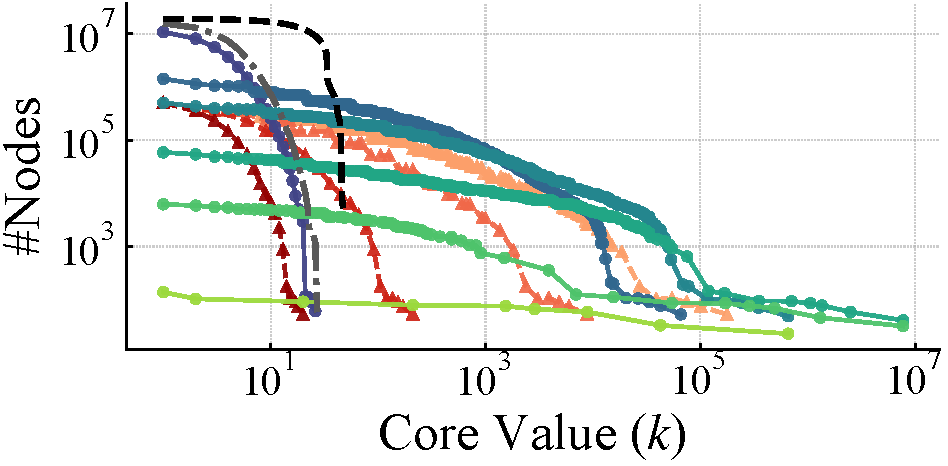
\includegraphics[width=0.47\linewidth]{figure/pokec_fused_nodes.pdf}
        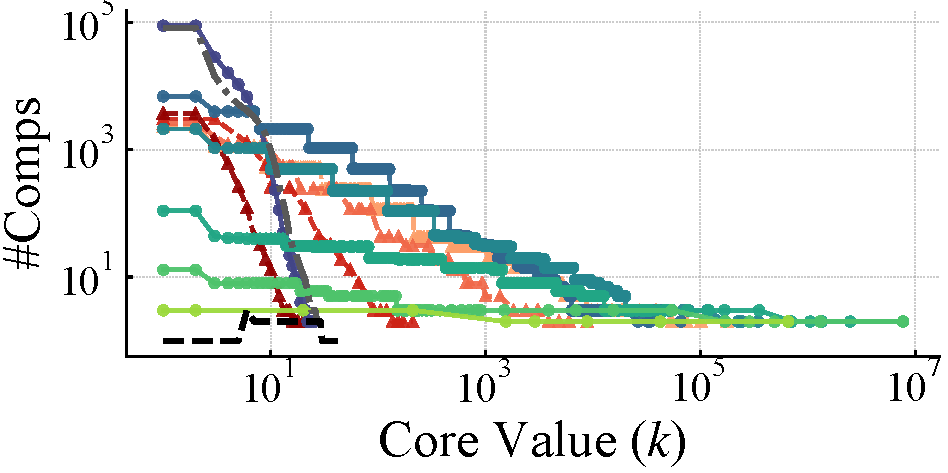
\includegraphics[width=0.47\linewidth]{figure/pokec_fused_comps.pdf}
        
        \captionof{figure}{Case study on \texttt{soc-pokec}. Solid (o): varying $s$; dashed ($\triangle$): varying $r$.}
        \label{fig:pokec-fused}
    \end{figure}

    % 右侧部分：collaborative network
    \begin{figure}
        \centering
        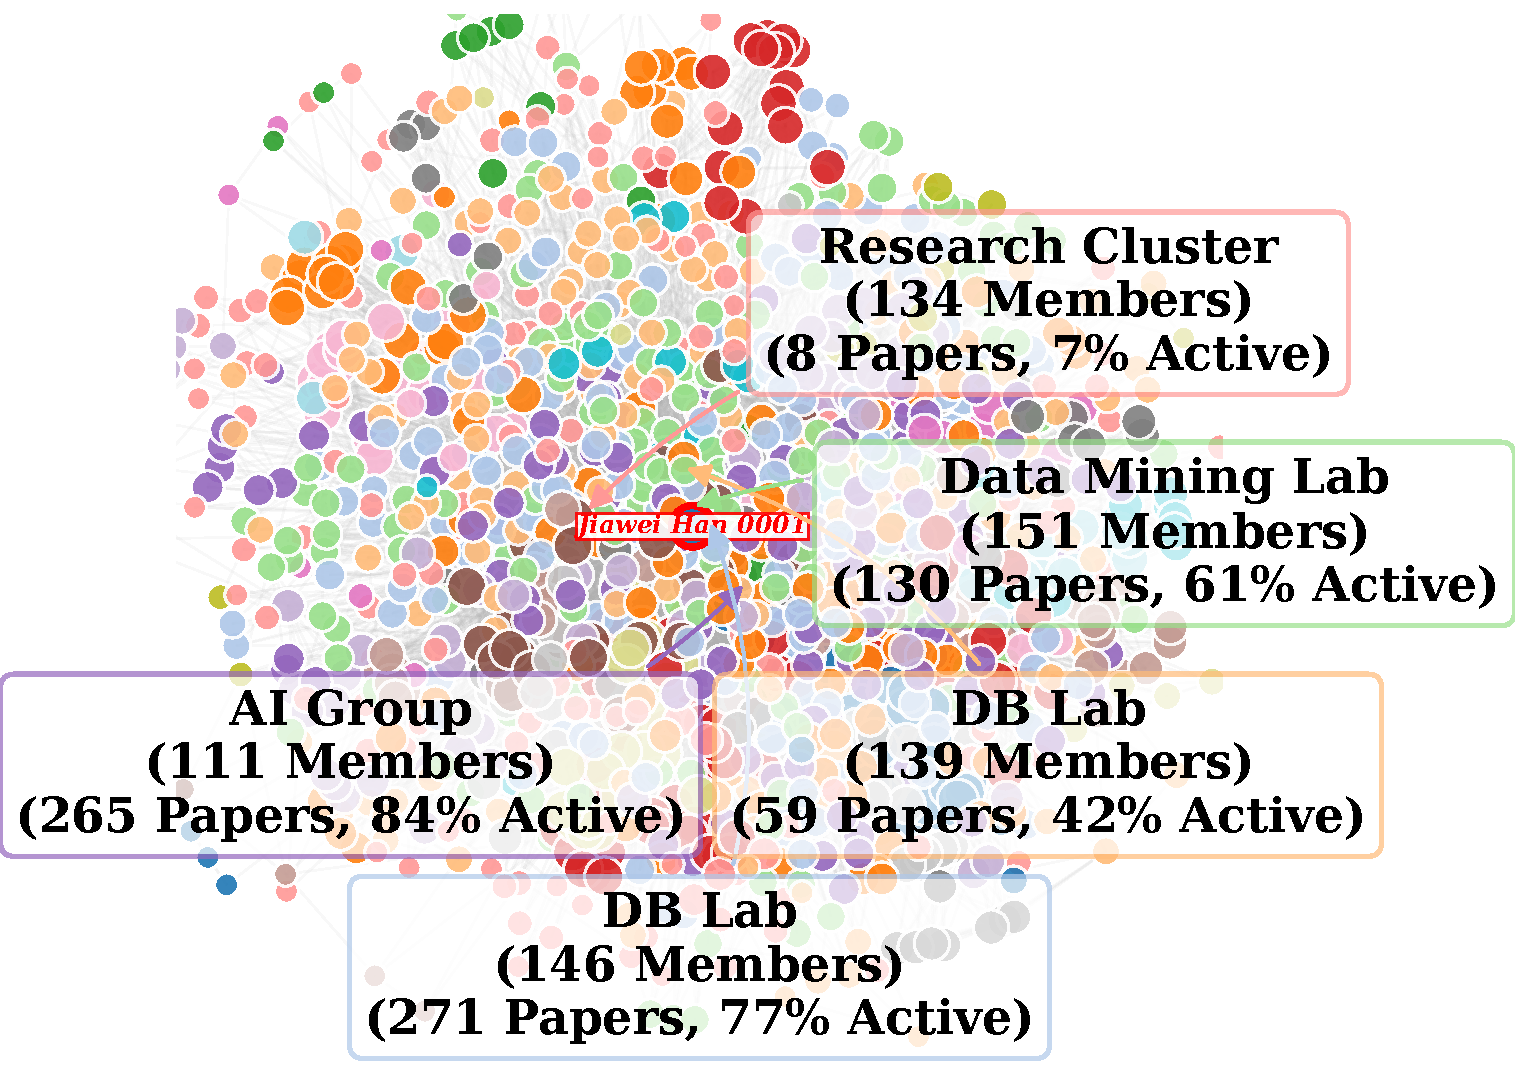
\includegraphics[width=0.47\linewidth]{figure/viz_collab_r3_s4.pdf} 
        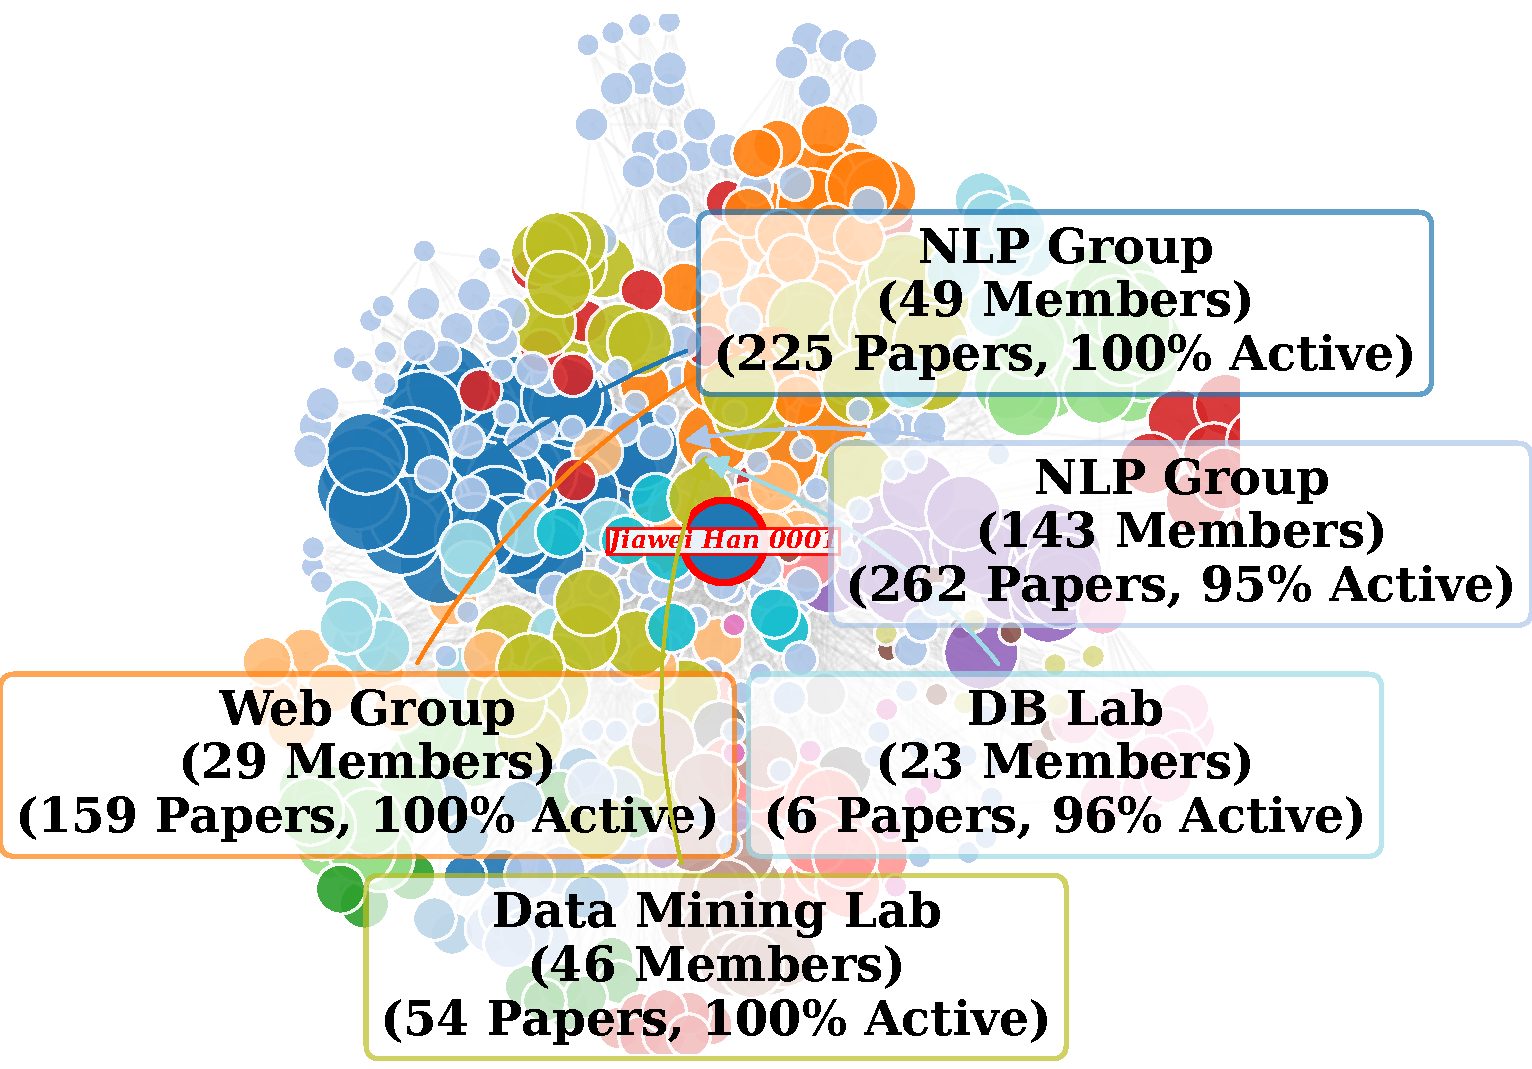
\includegraphics[width=0.47\linewidth]{figure/viz_collab_r3_s10.pdf} 
        
        \captionof{figure}{Case Study on Collaborative network: (a) Low Quality, (b) High Purity.}
        \label{fig:han-ego}
    \end{figure}
% \end{figure}

% \expsection{Case Study I: Parameter Sensitivity on \texttt{soc-pokec}}
% \label{sec:case-study-pokec}
% % 
% We examine how the two parameters---clique order $r$ and support threshold $s$---control the granularity of $(r,s)$-nucleus cores on \texttt{soc-pokec}.
% For each core value $k$ along the decomposition, we report (i) the number of surviving vertices (\texttt{living\_nodes})
% and (ii) the number of connected components (\texttt{components}) in the remaining nucleus subgraph.
% We include $k$-core ($r{=}1$) and $k$-truss ($r{=}2$) as standard baselines.

% \expsubsection{Varying $r$ under fixed $s$.}
% Fixing $s{=}10$, increasing $r$ provides limited and sometimes unstable simplification at typical operating points.
% At $k\ge 10$, moving from $r{=}3$ to $r{=}6$ reduces surviving vertices only from 319,139 to 233,661 ($1.37\times$),
% while the number of components slightly increases from 495 to 543.
% Even at a stronger threshold $k\ge 100$, $r{=}3$ retains 185,748 vertices with 226 components, whereas $r{=}6$ retains 52,041 vertices with 43 components.

% \expsubsection{Varying $s$ under fixed $r$.}
% Fixing a moderate clique order $r{=}3$, increasing $s$ yields order-of-magnitude pruning at the \emph{same} core threshold.
% At $k\ge 10$, the surviving vertices drop from 319,139 ($s{=}10$) to 42,435 ($s{=}14$) and further to 4,828 ($s{=}18$),
% while components drop from 495 to 40 and 8, respectively.
% The same trend holds at $k\ge 100$: 185,748 ($s{=}10$) $\rightarrow$ 22,017 ($s{=}14$) $\rightarrow$ 2,867 ($s{=}18$) vertices,
% and 226 $\rightarrow$ 20 $\rightarrow$ 5 components.

% \sstitle{Practical guideline (size-driven tuning).}
% We further quantify usability by the minimum core value $k_{\min}$ needed to obtain a compact subgraph.
% For $r{=}3$, achieving $\le 10{,}000$ vertices requires $k_{\min}{=}9714$ at $s{=}10$, but only $k_{\min}{=}1431$ at $s{=}14$,
% and already $k_{\min}{=}1$ at $s{=}18$ (6,252 vertices).
% Overall, on \texttt{soc-pokec}, tuning $s$ is a substantially more effective knob than tuning $r$ for distilling large cores into compact,
% well-structured modules; we thus recommend fixing a moderate $r$ (e.g., $r{=}3$) and using $s$ to control granularity.

\expsection{Case Study I: Parameter Sensitivity on \texttt{soc-pokec}}
\label{sec:case-study-pokec}
We study how $r$ and $s$ control the granularity of $(r,s)$-nucleus cores on \texttt{soc-pokec} (Figure~\ref{fig:pokec-fused}).
For each core value $k$, we report the number of surviving vertices and connected components in the remaining nucleus subgraph, and include $k$-core ($r{=}1, s{=}2$) and $k$-truss ($r{=}2, s{=}3$) as baselines.
Since the absolute scale of $k$ varies across $(r,s)$, we compare different settings mainly at the same \emph{rank} of $k$ along each curve.

\sstitle{Varying $r$ with fixed $s$.}
With $s{=}10$, at the 25\%-$k$ rank, $r{=}3$ keeps 141{,}392 vertices with 110 components, while $r{=}6$ keeps 148{,}295 vertices but increases to 245 components.

\sstitle{Varying $s$ with fixed $r$.}
Fix $r{=}3$ and increase $s$ from 10 to 14 to 18.
At the 10\%-$k$ rank (a typical operating regime), the remaining subgraph shrinks from
195{,}278 vertices / 226 components ($s{=}10$) to
32{,}310 / 30 ($s{=}14$) and further to
5{,}009 / 8 ($s{=}18$).
At the median $k$ rank, vertices drop from
78{,}233 / 41 ($s{=}10$) to
11{,}325 / 14 ($s{=}14$) and
2{,}867 / 5 ($s{=}18$).

\sstitle{$k$-core and $k$-truss (low-order baselines).}
At the 10\%-$k$ rank, $k$-core retains $18{,}449{,}233$ vertices in a single component, which is too coarse to separate modules.
$k$-truss retains $10{,}138{,}083$ vertices but yields $14{,}286$ components, indicating that low-order $(2,3)$ support admits many residual structures.
By contrast, $(r,s)=(3,10)$ at the same rank retains $195{,}278$ vertices and $226$ components, producing substantially more compact and well-structured modules.


\sstitle{The benefit of tuning $s$.}
Increasing $s$ reduces both the surviving size and the number of components, producing compact and well structured modules. It theoretically filters out incidental structures.


\sstitle{Practical guideline.}
We recommend fixing a moderate $r$ (e.g., $r{=}3$) and tuning $s$ to control granularity.
% 但是当s过大的时候, 图中获取的信息可能会过少, 例如在s=22的情况下, 大部分的节点都被删除了, 只剩下非常少的节点和连通分量.
% When $s$ is too large, close to the maximum clique size(29), the remaining subgraph may become too small to be informative (e.g., at $s{=}22$, 
When $s$ is too large(s=22), close to the dataset's maximum clique size (29), very few $s$-cliques exist and the remaining subgraph may become too small to be informative, most nodes are removed, leaving only a few nodes and components.




% \expsection{Case Study II: Ego Network of Jiawei Han on DBLP}
% \label{sec:case-study-han}
% We study a real collaboration ego network centered at Jiawei Han (1-hop coauthor graph).
% Using fixed clique order $r{=}3$, we compare two support thresholds ($s{=}4$ vs.\ $s{=}10$).
% A node is considered \emph{surviving} if its nucleus core value is positive; nodes are colored by the connected nucleus component (\texttt{cluster\_id}).
% For each component $C$, we further quantify collaboration strength using the DBLP paper list:
% a paper is counted as \emph{collaborative within $C$} if it contains at least
% $\tau(C)=\min\{5,\max(3,\lfloor 0.1|C|\rfloor)\}$ authors from $C$; the participation ratio is the fraction of members that appear in such papers.

% \ssstitle{Large $s$ yields compact and well-separated collaboration modules.}
% Increasing $s$ from 4 to 10 reduces the surviving subgraph from 1,328 to 540 nodes (59.3\%) and from 65 to 27 components (58.5\%),
% while the fraction of intra-component edges increases from 0.319 to 0.528.
% Structural quality improves substantially: the size-weighted average separability $m_{\mathrm{in}}/m_{\mathrm{cut}}$
% increases from 0.270 to 0.750, and conductance $m_{\mathrm{cut}}/(2m_{\mathrm{in}}+m_{\mathrm{cut}})$ drops from 0.712 to 0.475.

\expsection{Case Study II: Identifying ego network on DBLP.}
\label{sec:case-study-han}
We study Jiawei Han's 1-hop coauthor ego graph on DBLP and compare $s{=}4$ vs.\ $s{=}10$ under $r{=}3$.
In Fig.~\ref{fig:han-ego}, nodes are colored by nucleus component and we annotate the top-$5$ largest ones.
For each surviving component $C$, let $m_{\mathrm{in}}$ be the number of internal edges and $m_{\mathrm{cut}}$ the number of edges from $C$ to other surviving components.
We report $\phi(C)=m_{\mathrm{cut}}/(2m_{\mathrm{in}}+m_{\mathrm{cut}})$ and $m_{\mathrm{in}}/m_{\mathrm{cut}}$; lower $\phi(C)$ and higher $m_{\mathrm{in}}/m_{\mathrm{cut}}$ indicate better separation.
Using DBLP paper lists restricted to this ego network, a paper is \emph{collaborative} for $C$ if it contains $\ge3$ authors from $C$, and the \emph{active ratio} is the fraction of members appearing in at least one collaborative paper.


\sstitle{Larger $s$ yields compact and better-separated modules.}
Increasing $s$ from $4$ to $10$ shrinks the surviving subgraph from $1{,}328$ to $540$ nodes and reduces components from $65$ to $27$,
while increasing the intra-component edge fraction from $0.319$ to $0.528$.
The size-weighted average separability improves from $0.270$ to $0.750$, and the conductance score drops from $0.712$ to $0.475$,
showing that larger $s$ produces more cleanly separated collaboration modules.

\sstitle{Larger $s$ preserves highly active.}
Under the same collaboration threshold (3 within-component coauthors), the top-$5$ annotated components at $s{=}4$
have an average active ratio of $54.25\%$, and already exhibit a clear long tail (e.g., a $134$-member component has only $8$ collaborative papers and $7\%$ active members).
In contrast, at $s{=}10$ the top-$8$ components have an average active ratio of $98.15\%$; most are near $100\%$ active, with the smallest $95\%$.
This indicates that increasing $s$ filters loosely coordinated/noisy groups and retains compact, strongly collaborating teams that are easier to interpret.



% improving separability from $0.326$ to $0.666$.
% Overall, among components with at least one collaborative paper, node-level participation increases from $0.650$ to $0.901$,
% and the node share with participation $\ge 0.8$ rises from $0.453$ to $0.732$,
% supporting that tuning $s$ is an effective knob for extracting compact and interpretable collaboration cores.
